\chapter{Análise e Exploração dos Dados}

Nesta etapa da analise dos dados, uma das primeiras informações que levantamos foi a quantidade de estações por estado. Na Figura \ref{fig:estacoes_por_estado} podemos observar que os estados com maior quantidade de estações meteorológicas instalados são, em primeiro lugar, Minas Gerais com 116 estações, seguido pelos estados da Bahia com 78 estações,  Rio Grande do Sul com 62 estações e São Paulo com 54 estações. Em contrapartida, os estados de Rondônia,  Roraima, e Amapá possuem apenas 7, 5 e 5 estações, respectivamente.  

\begin{figure}[H]
    \centering
    \caption{Distribuição, por estado, das estações meteorológicas analisadas.}
    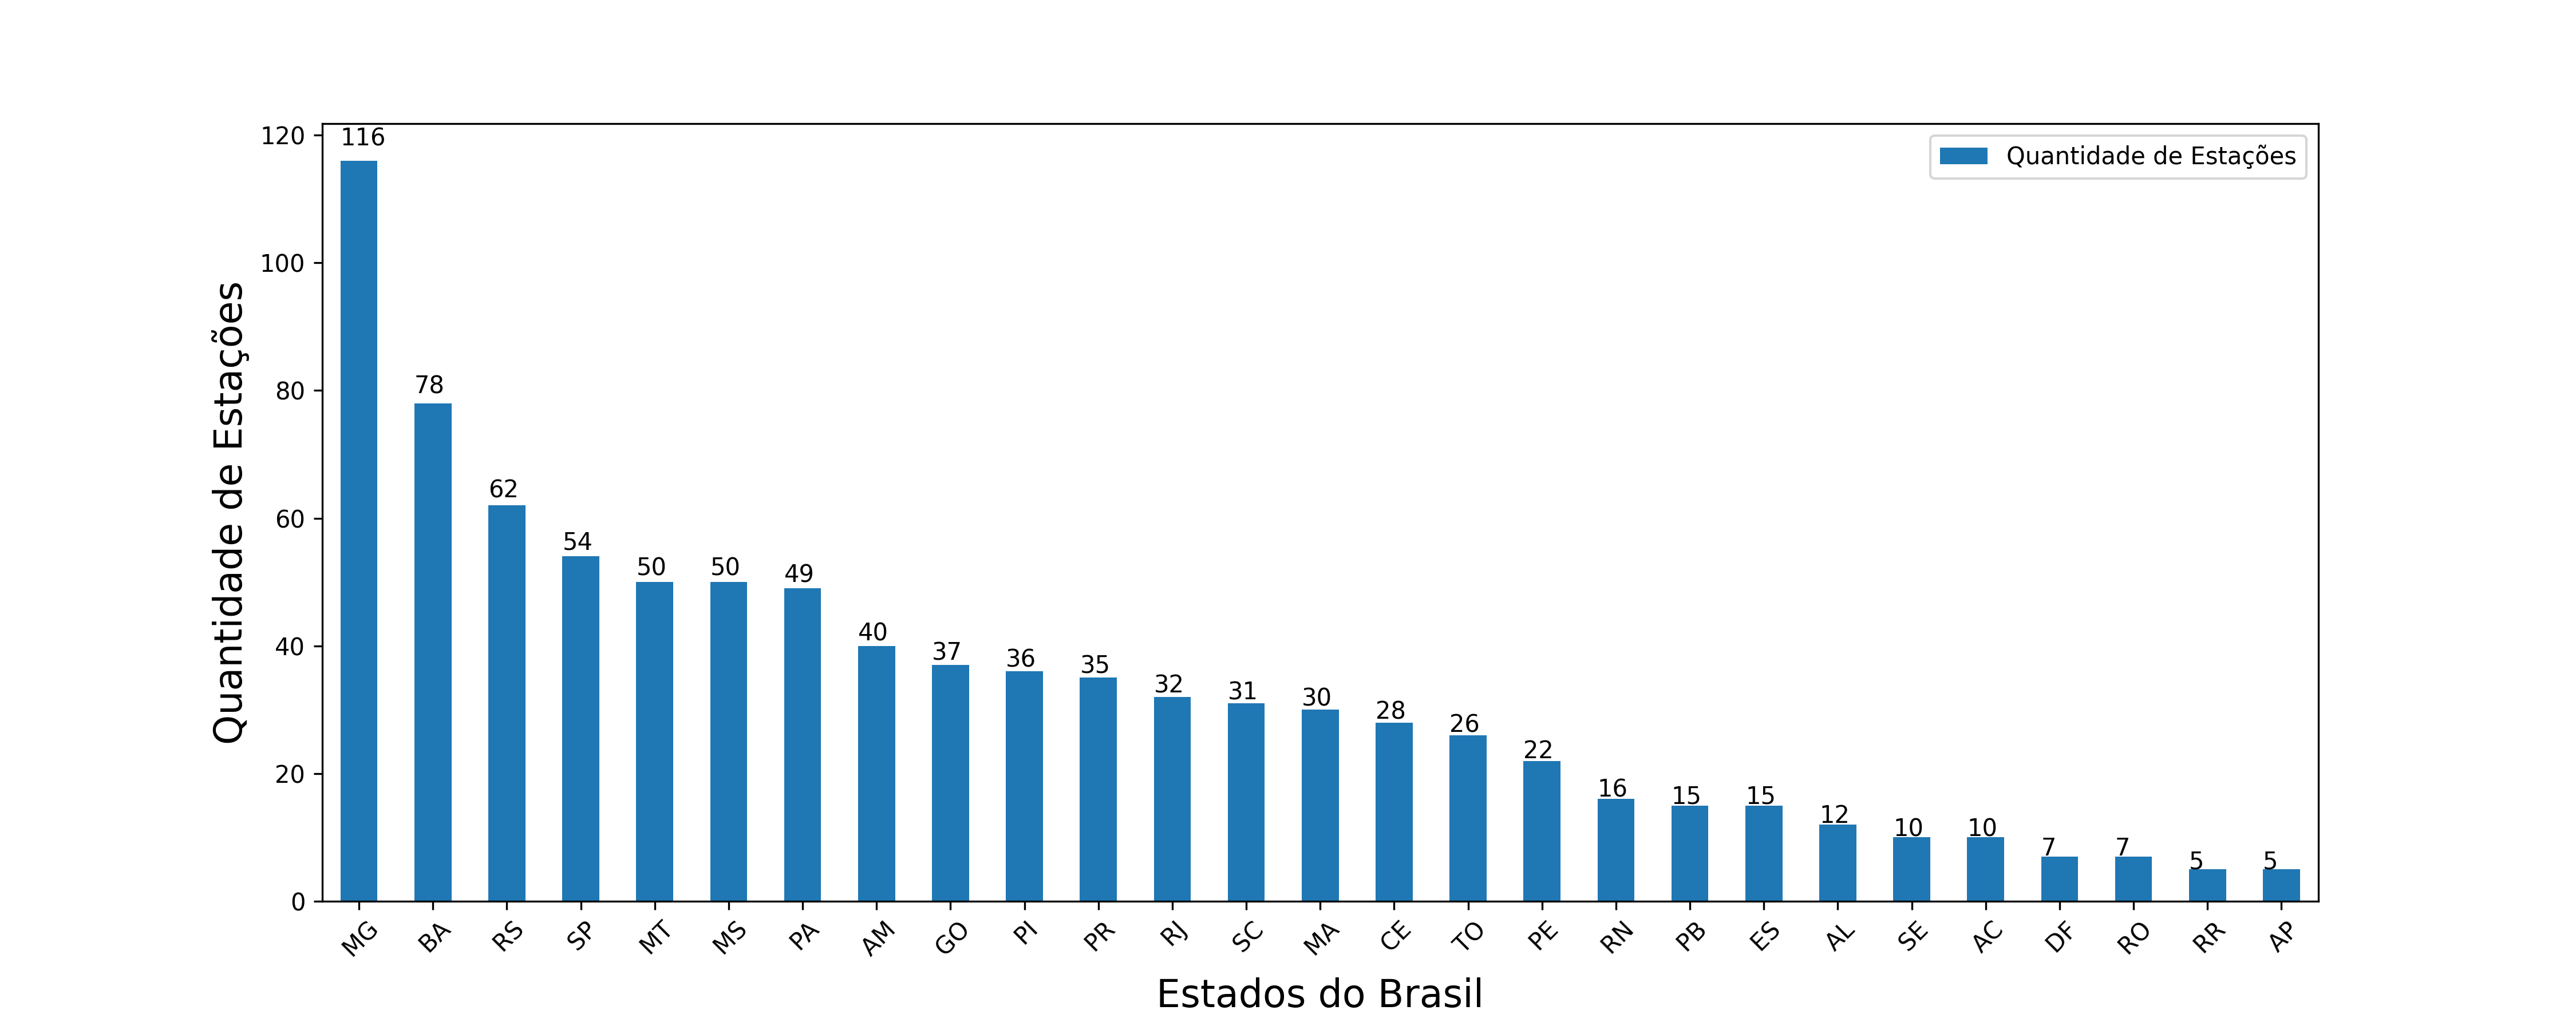
\includegraphics[width=0.9\textwidth]{figuras/estacoes_por_estado.png}
    \label{fig:estacoes_por_estado}
\end{figure}

Dentre estas estações analisadas, há estações convencionais com dados disponíveis deste do ano de 1961, até estações automáticas recentemente instaladas, com dados apenas para os últimos anos. Por isso, é importante entendermos como varia a disponibilidade de dados ao longo de todo o período afim de nos orientarmos melhor na criação dos nossos modelos. Para isso, apresentamos na Figura \ref{fig:disponibilidade_historica_de_dados} a disponibilidade das observações das estações ao longo de todo o período analisado. Podemos observar que a partir do ano de 2002 há um crescimento na quantidade de dados disponíveis, com maiores crescimentos nos anos de 2007 e 2008. Isso se deve pela adoção ao processo de automação de dados meteorológicos através de monitoramento por estacões automáticas que surgiu no Brasil no inicio deste século.  

\begin{figure}[H]
    \centering
    \caption{Disponibilidade de dados ao longo de todo o período analisado.}
    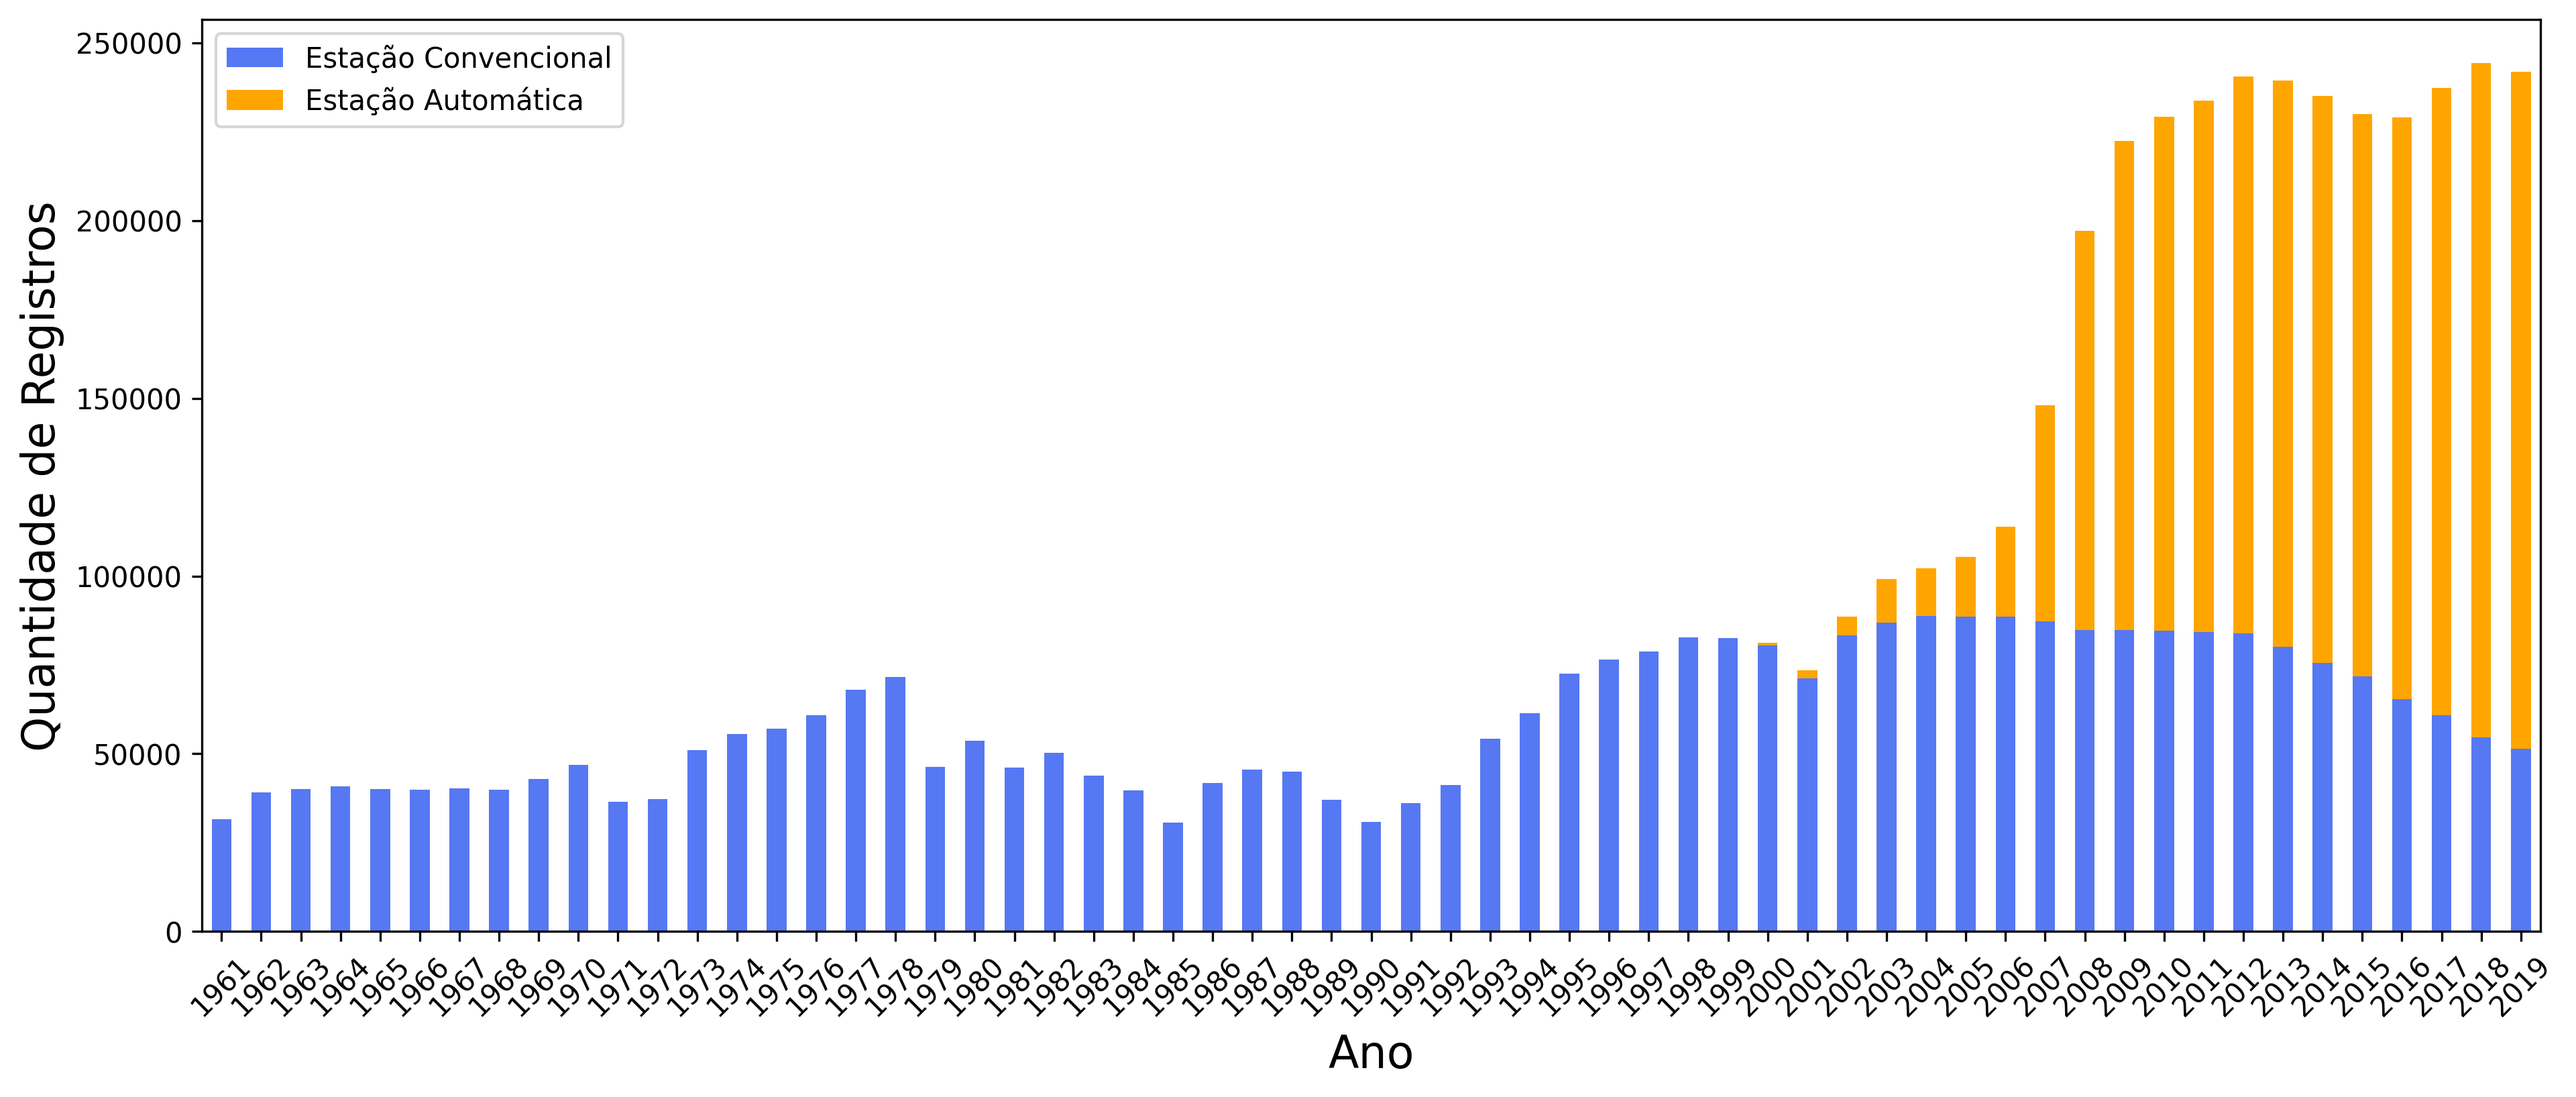
\includegraphics[width=0.9\textwidth]{figuras/disponibilizade_historica_de_dados.png}
    \label{fig:disponibilidade_historica_de_dados}
\end{figure}

Ainda observando a Figura \ref{fig:disponibilidade_historica_de_dados}, é possível observarmos uma declínio de dados em alguns anos específicos. Por exemplo, de 1978 para 1979 houve uma diminuição na quantidade de dados disponíveis. Para entender melhor essa variação, e avaliar melhor a quantidade de dados que ficaram ausentes no conjunto final, adicionamos na Figura \ref{fig:dados_ausentes_ao_longo_anos} também a quantidade de dados que estão ausentes para os anos apresentados.

\begin{figure}[H]
    \centering
    \caption{Disponibilidade de dados ao longo de todo o período analisado.}
    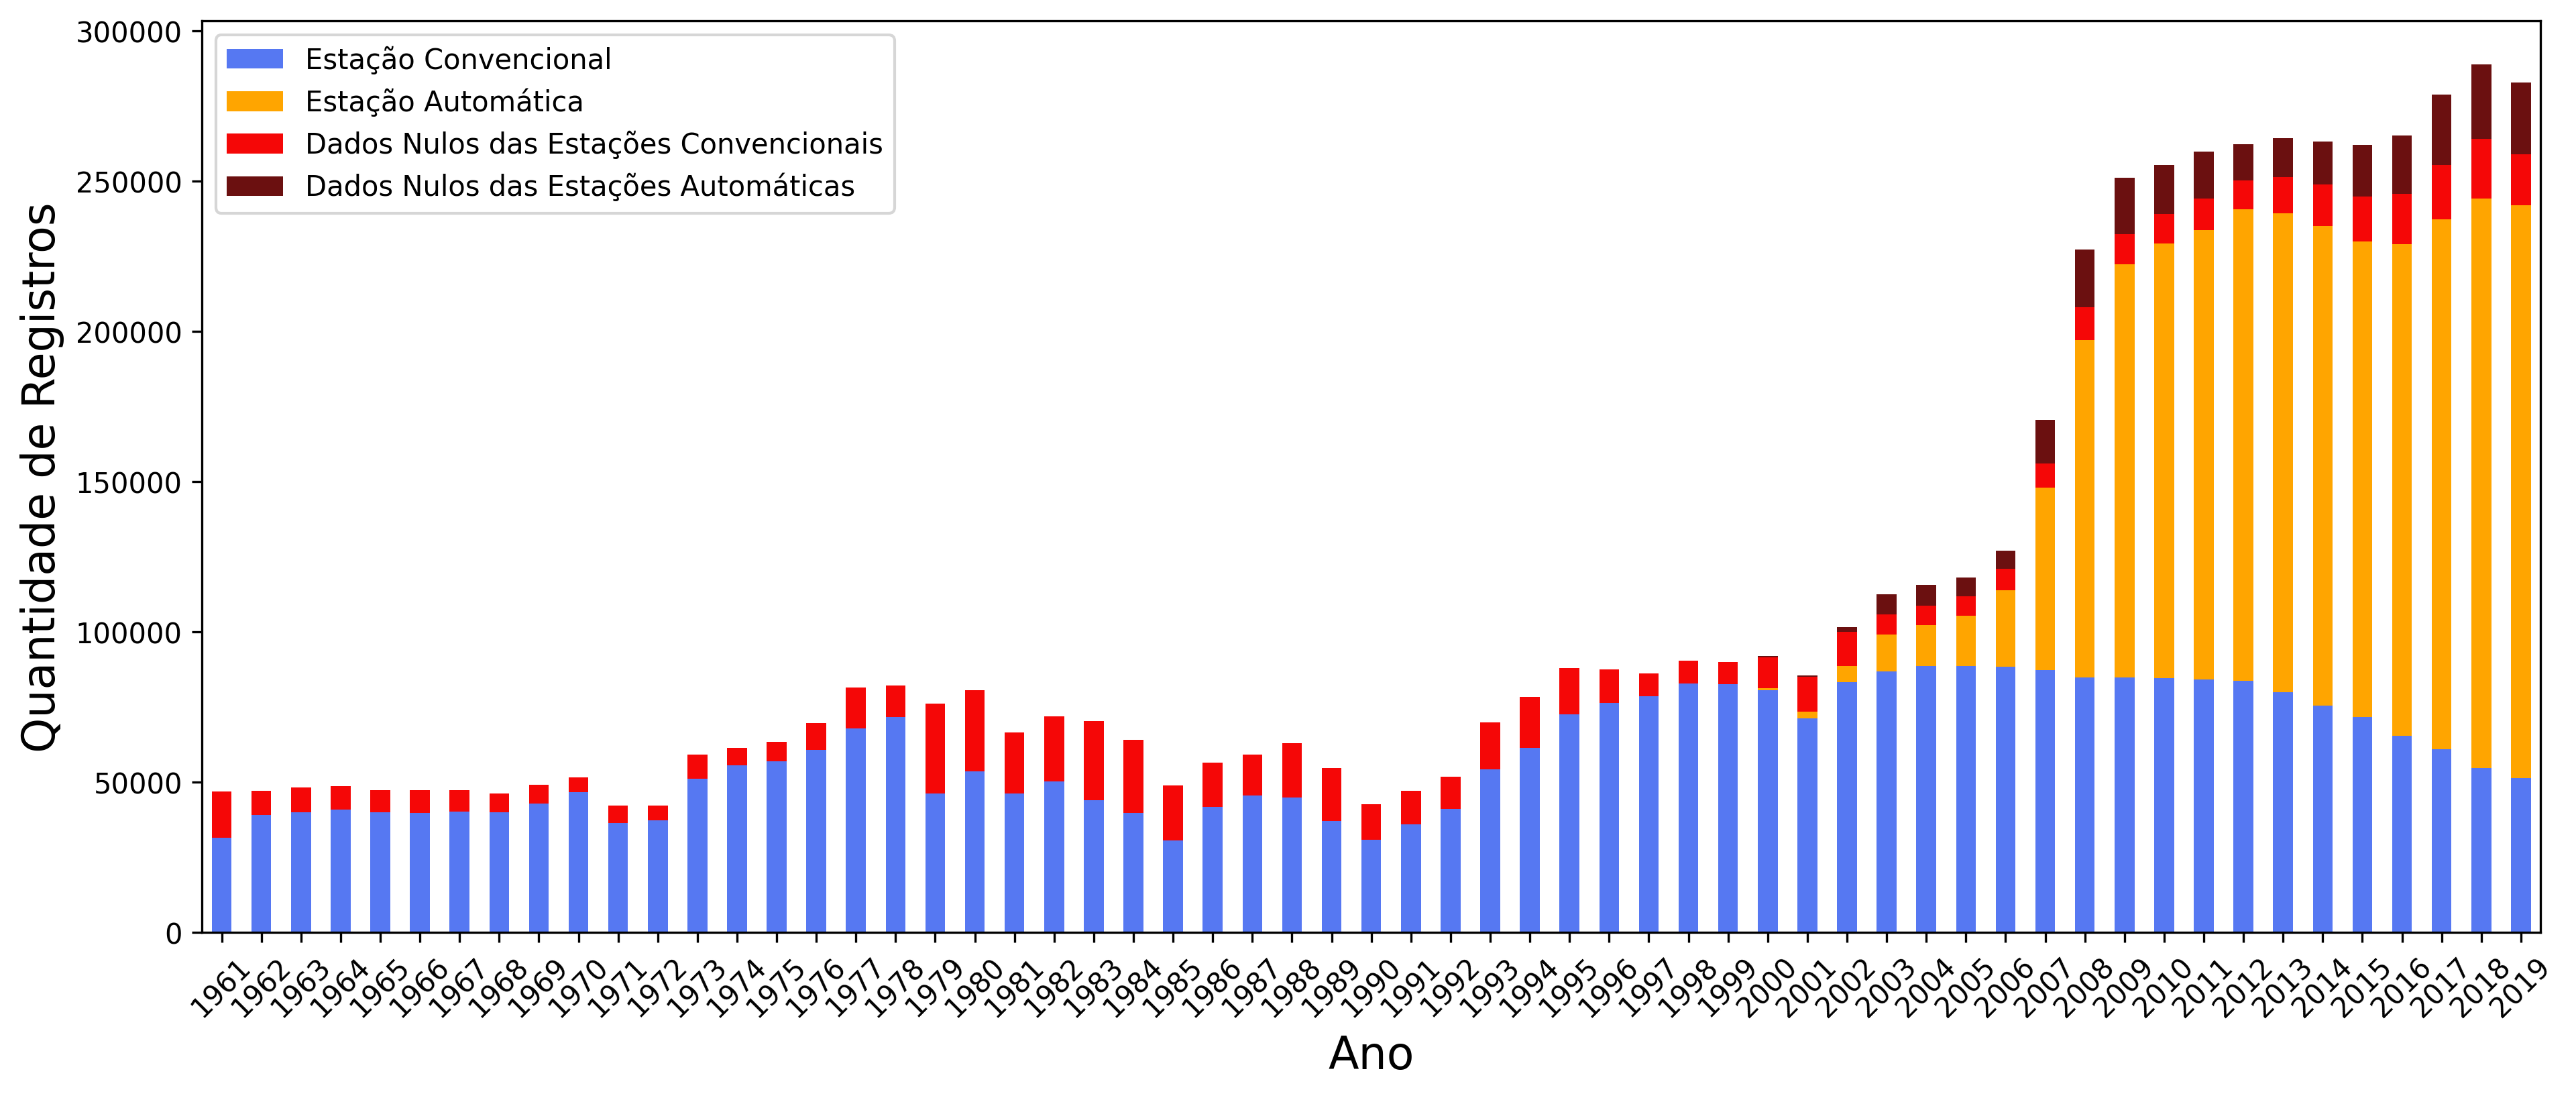
\includegraphics[width=0.9\textwidth]{figuras/dados_ausentes_ao_longo_anos.png}
    \label{fig:dados_ausentes_ao_longo_anos}
\end{figure}

A ausência de dados em estações meteorológicas pode ser causada por várias razões, entre elas mudança geográfica da estação, mudança no instrumental, tempo de observação e práticas observacionais utilizadas \cite{oliveira2019estaccao}. 

Uma informação que também é importante identificarmos nos dados, é se, valores extremos que ocorreram, de fato, na realidade, não foram removidos durante o processo de limpeza dos dados.
Para isso, ilustramos nas Figuras \ref{fig:estacoes_convencionais_maiores_temperaturas} e \ref{fig:estacoes_convencionais_menores_temperaturas} os recordes de temperatura máxima e mínima para as estações convencionais do INMET, pois estas são as que possuem maior série histórica e maior consistência dos valores. 

\begin{figure}[H]
    \centering
    \caption{Recorde das maiores temperaturas já registradas no período de 1961 a 2019 nas estações convencionais do INMET.}
    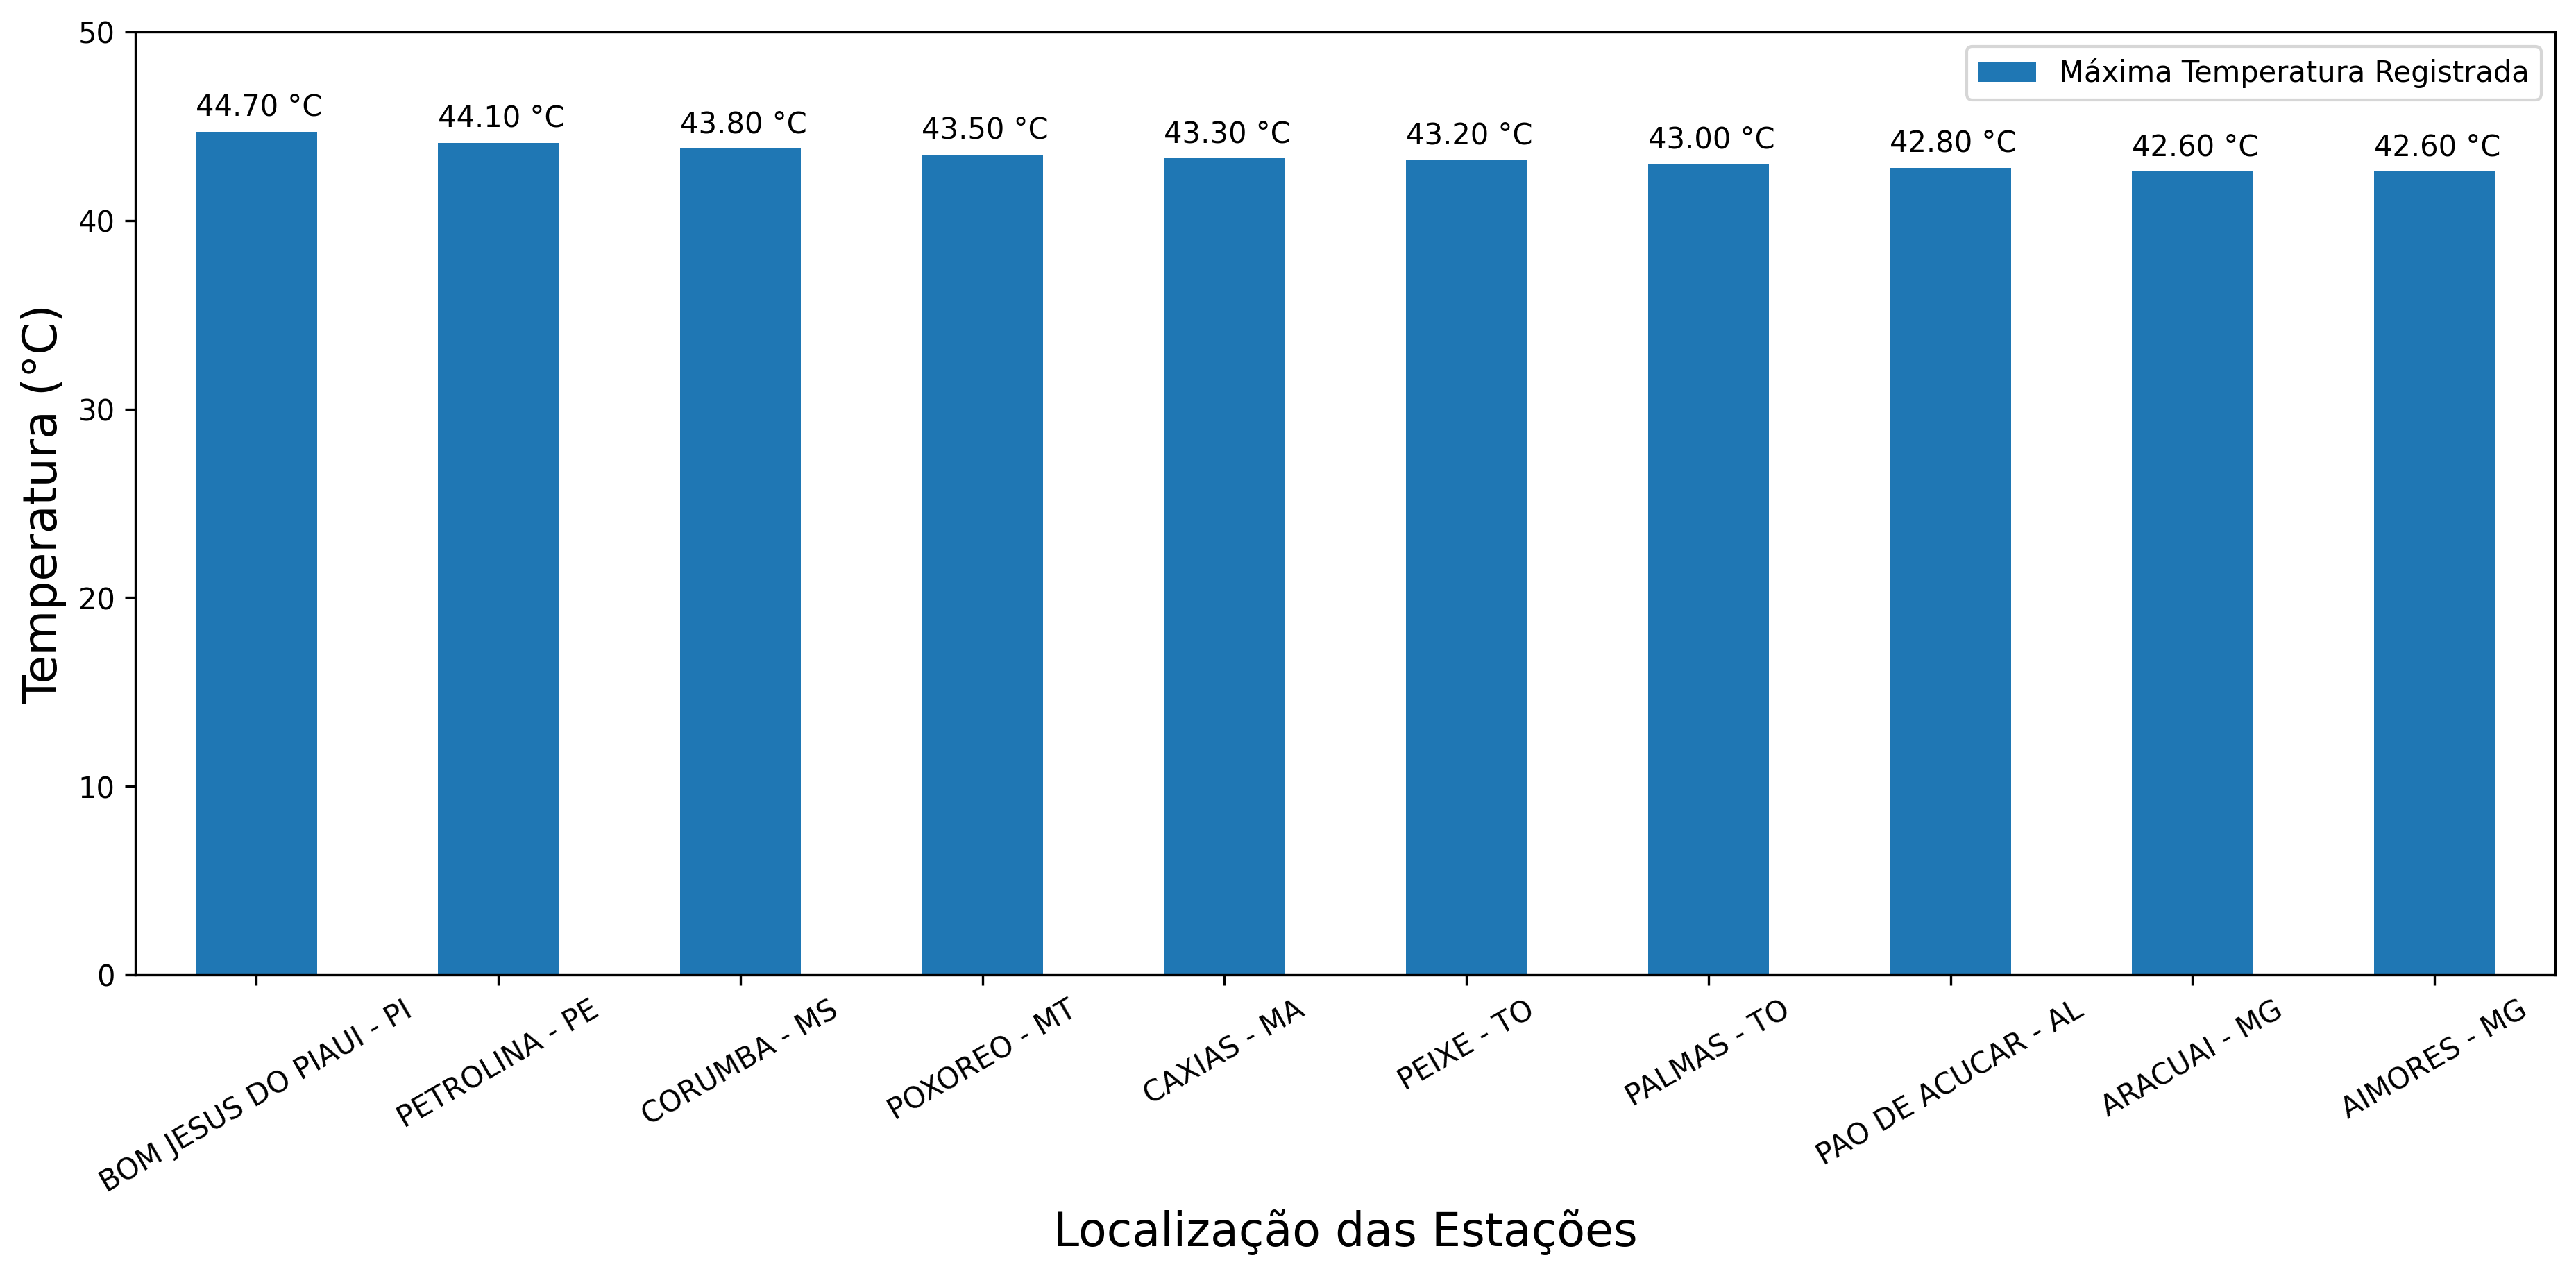
\includegraphics[width=0.9\textwidth]{figuras/estacoes_convencionais_maiores_temperaturas.png}
    \label{fig:estacoes_convencionais_maiores_temperaturas}
\end{figure}

\begin{figure}[H]
    \centering
    \caption{Recorde das menores temperaturas já registradas no período de 1961 a 2019 nas estações convencionais do INMET.}
    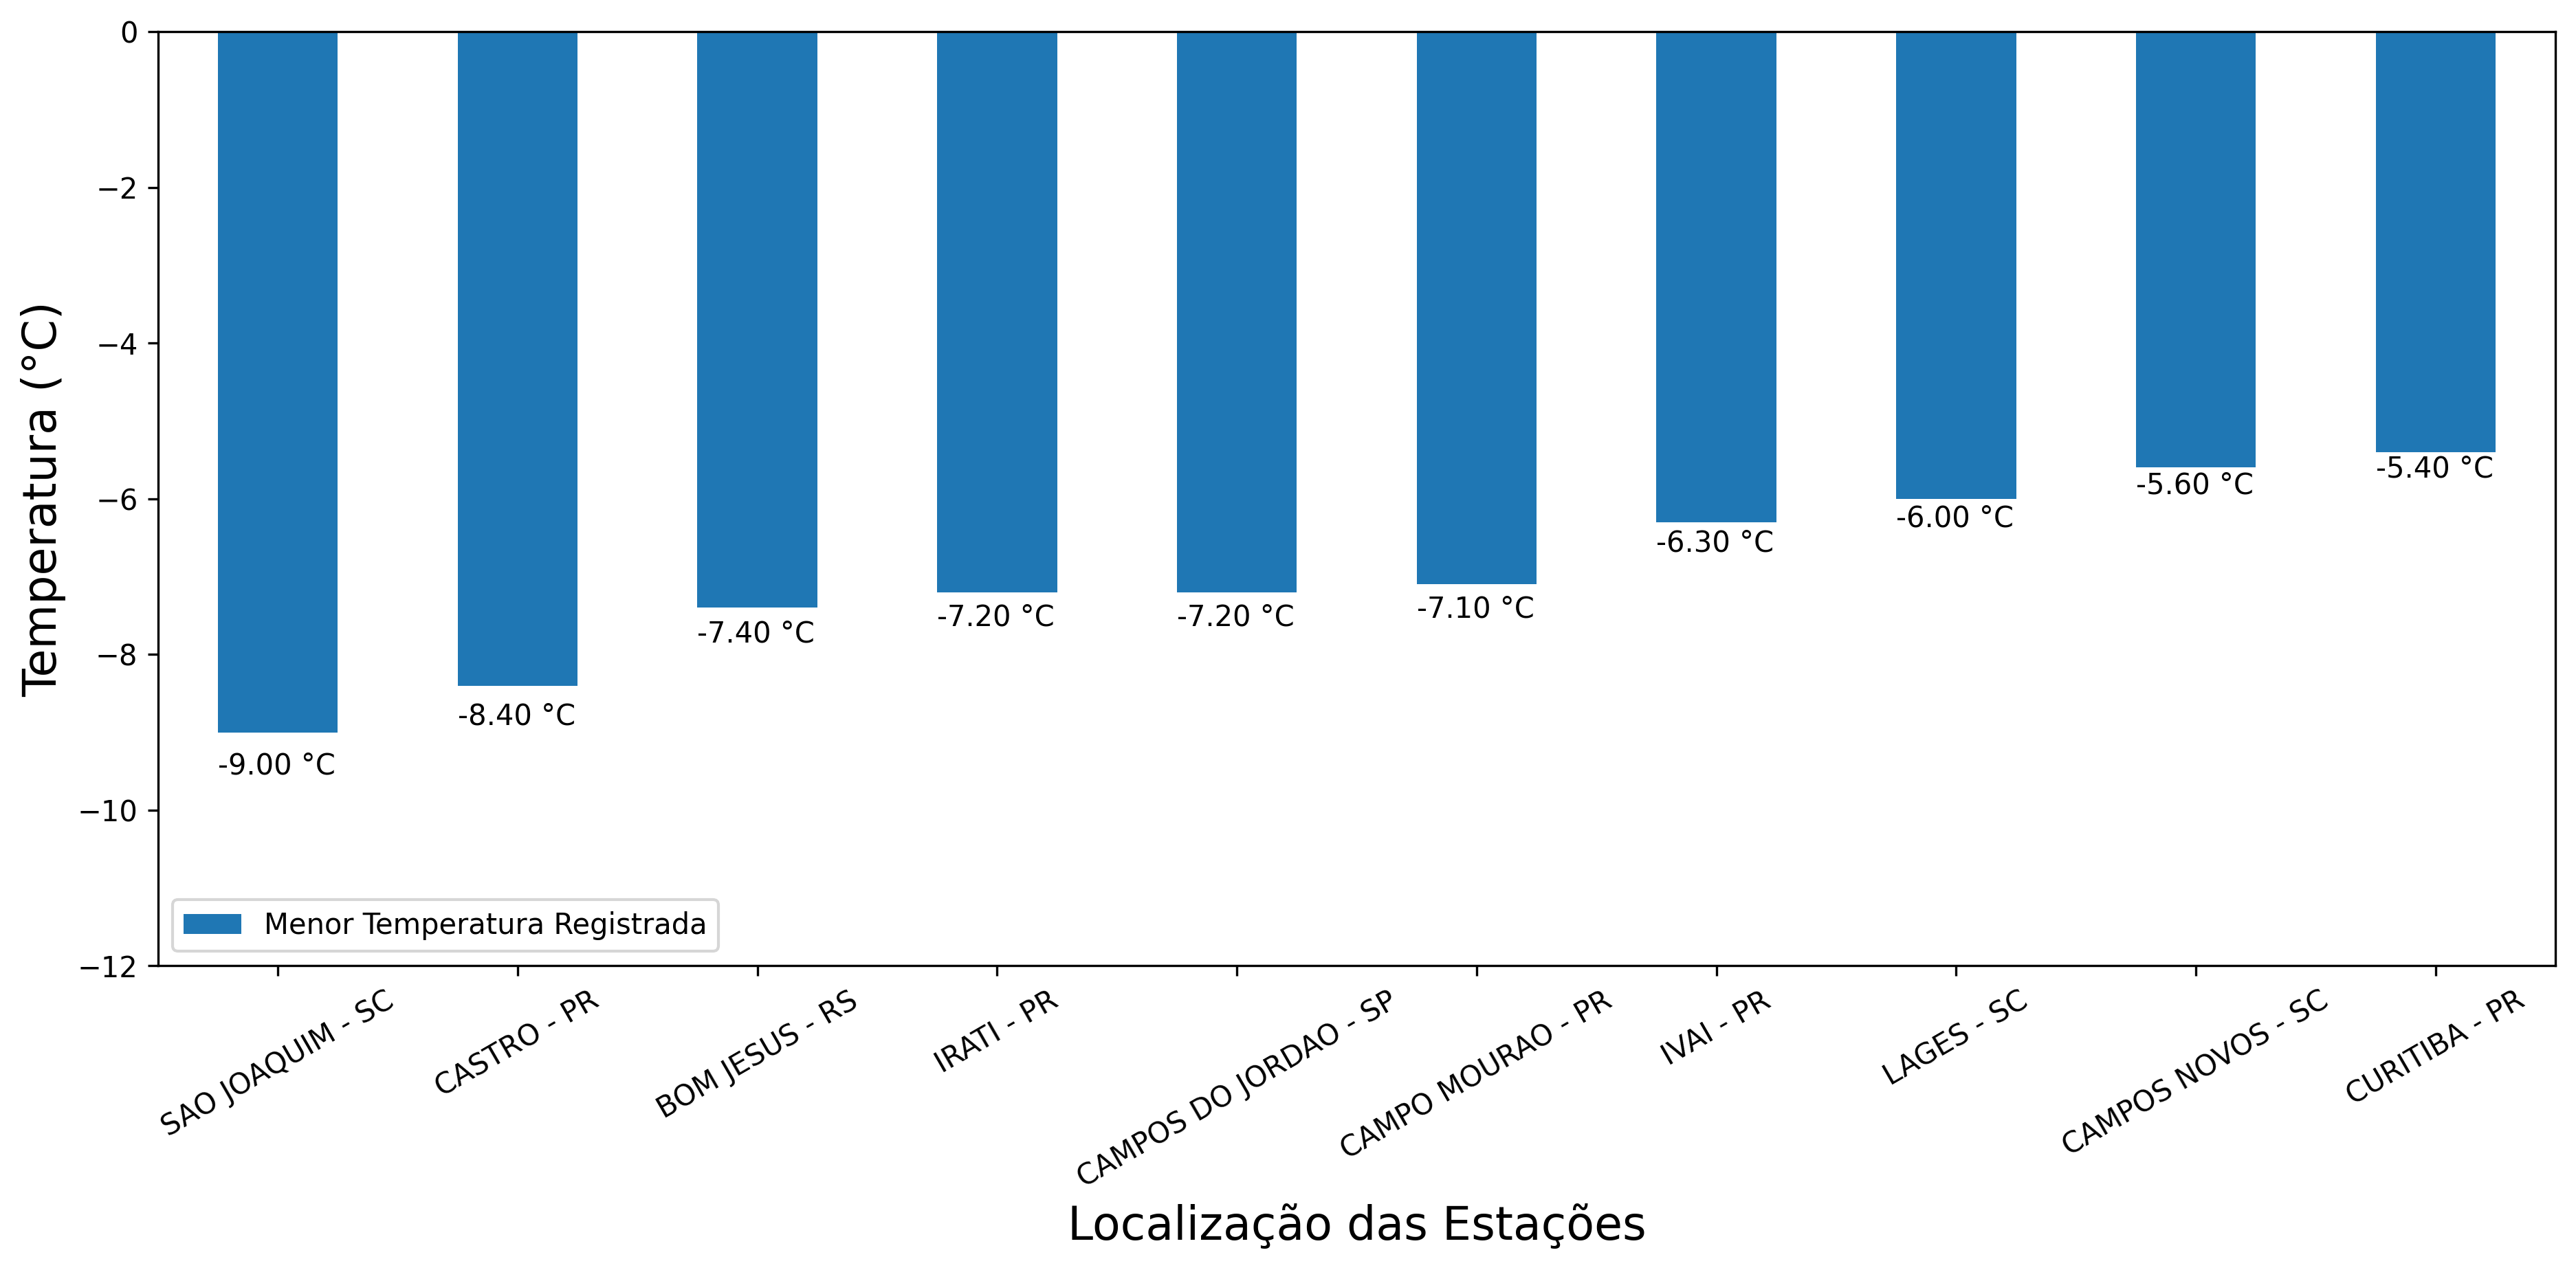
\includegraphics[width=0.9\textwidth]{figuras/estacoes_convencionais_menores_temperaturas.png}
    \label{fig:estacoes_convencionais_menores_temperaturas}
\end{figure}

Realizando uma pesquisa na internet sobre os recordes de temperatura no Brasil encontramos as seguintes informações: 

\begin{displayquote}
"A maior temperatura registrada oficialmente no Brasil foi 44,7 $^{\circ}$C em Bom Jesus, Piauí, em 21 de novembro de 2005, superando o recorde também oficial de Orleans, Santa Catarina, de 44,6 $^{\circ}$C, de 6 de janeiro de 1963. Já a menor temperatura registrada foi de -17,8 $^{\circ}$C no Morro da Igreja, em Urubici, Santa Catarina, em 29 de junho de 1996 (registro extraoficial). A menor temperatura registrada oficialmente no país foi de -14 $^{\circ}$C, no município de Caçador, no mesmo estado, em 11 de junho de 1952." \cite{wiki:clima_do_brasil}.
\end{displayquote}

Essa referência aponta o município de Bom Jesus, no estado do Piauí, com a maior temperatura já registrada no Brasil, com a temperatura alcançando 44,70 $^{\circ}$C em 21 de novembro de 2005, exatamente como os dados das estações convencionais apresentaram.  Também segundo a referência, a menor temperatura já registrada após 1961 foi de -17,8 $^{\circ}$C no Morro da Igreja, em Urubici, Santa Catarina, em 29 de junho de 1996. Analisando os dados, diferente do que apontou a informação encontrada, a menor temperatura registrada pelas estações convencionais foi no município de São Joaquim, em Santa Catarina. Cruzando o mapa de municípios de Santa Catarina com as estações que estamos analisando, observamos que o município de São Joaquim faz fronteira com o município de Urubici e que, dos dois municípios, apenas o de São Joaquim possui, nos dados analisados, estações meteorológicas, o que indica um possível motivo das diferenças entre as informações.